% Étape 6 : l'encodeur complet, L couches, deux images, les mêmes poids (FreeFlow)
% Compiler avec pdflatex (ou Overleaf).
\documentclass[border=10pt]{standalone}
\usepackage[T1]{fontenc}
\usepackage[utf8]{inputenc}
\usepackage[scaled]{helvet}
\renewcommand{\familydefault}{\sfdefault}
\usepackage{sansmath}
\sansmath
\usepackage{amsmath}
\usepackage{tikz}
\usetikzlibrary{arrows.meta}

\definecolor{bleu}{HTML}{9CC8F0}     % X, image 1 et 2
\definecolor{rouge}{HTML}{F4A6A6}    % F, sortie
\definecolor{gris}{HTML}{CCCCCC}
\definecolor{grisclair}{HTML}{F2F2F2}
\definecolor{noir}{HTML}{222222}

\tikzset{
  th/.style={font=\fontsize{14}{16}\selectfont\bfseries, text=black, inner sep=0pt},
  ts/.style={font=\fontsize{12}{14}\selectfont, text=black, inner sep=0pt},
  tm/.style={font=\fontsize{13}{15}\selectfont, text=black, inner sep=0pt},
  fl/.style={noir, line width=1.4pt, -{Stealth[length=7pt]}},
}
\newcommand{\grid}[6]{%
  \fill[#6] (#1,#2) rectangle ++(#4*#5,#3*#5);
  \ifnum#4>1 \foreach \k in {1,...,\numexpr#4-1\relax} \draw[white, line width=1pt] (#1+\k*#5,#2) -- ++(0,#3*#5); \fi
  \ifnum#3>1 \foreach \k in {1,...,\numexpr#3-1\relax} \draw[white, line width=1pt] (#1,#2+\k*#5) -- ++(#4*#5,0); \fi}
% matrice N x D (4 x 4 cases de 10) : \mat{x}{y}{couleur}
\newcommand{\mat}[3]{\grid{#1}{#2}{4}{4}{10}{#3}}
% couche (boîte commune aux deux images) : \couche{x}{titre}{poids}
\newcommand{\couche}[3]{%
  \filldraw[fill=grisclair, draw=noir, line width=1pt, rounded corners=6pt] (#1,62) rectangle ++(100,236);
  \node[tm, anchor=base] at (#1+50,82) {#2};
  \node[ts, anchor=base] at (#1+50,176) {Win};
  \node[ts, anchor=base] at (#1+50,192) {$\downarrow$ Swin};
  \node[ts, anchor=base] at (#1+50,208) {$\downarrow$ Global};
  \node[ts, anchor=base] at (#1+50,288) {poids #3};
  \draw[fl] (#1+10,110) -- (#1+90,110);
  \draw[fl] (#1+10,250) -- (#1+90,250);}

\begin{document}
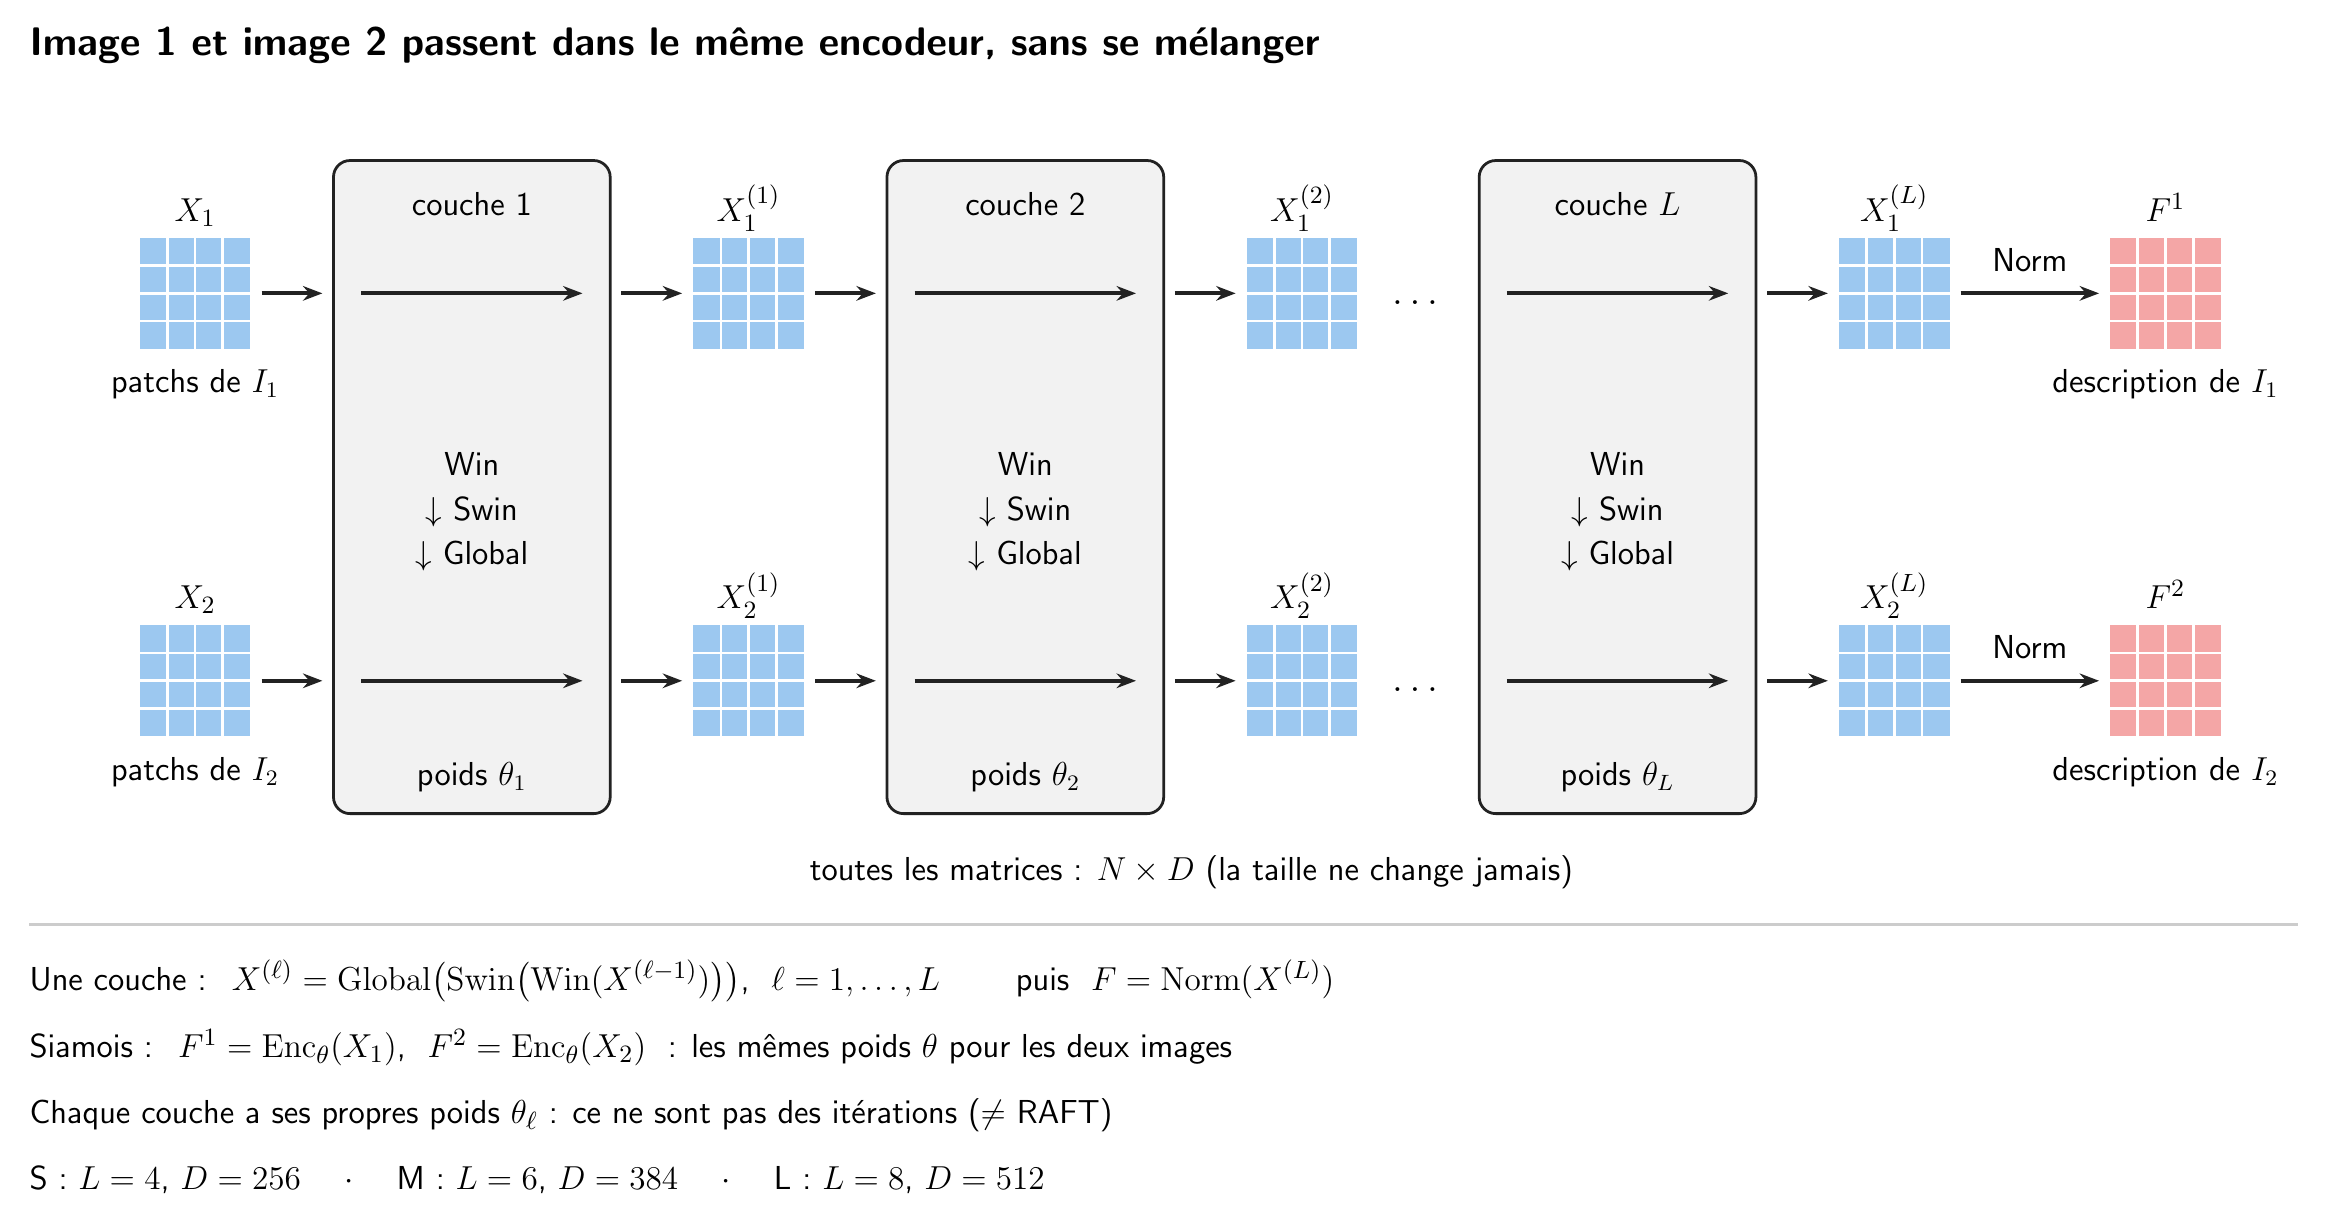
\begin{tikzpicture}[x=1pt, y=-1pt, line join=miter]

% étiquettes des deux pistes
\node[th, anchor=base west] at (0,24) {Image 1 et image 2 passent dans le même encodeur, sans se mélanger};

% entrées
\node[tm, anchor=base] at (60,84) {$X_1$};
\mat{40}{90}{bleu}
\node[ts, anchor=base] at (60,146) {patchs de $I_1$};
\node[tm, anchor=base] at (60,224) {$X_2$};
\mat{40}{230}{bleu}
\node[ts, anchor=base] at (60,286) {patchs de $I_2$};

% couche 1
\draw[fl] (84,110) -- (106,110);  \draw[fl] (84,250) -- (106,250);
\couche{110}{couche 1}{$\theta_1$}
\draw[fl] (214,110) -- (236,110); \draw[fl] (214,250) -- (236,250);
\node[tm, anchor=base] at (260,84) {$X_1^{(1)}$};
\mat{240}{90}{bleu}
\node[tm, anchor=base] at (260,224) {$X_2^{(1)}$};
\mat{240}{230}{bleu}

% couche 2
\draw[fl] (284,110) -- (306,110); \draw[fl] (284,250) -- (306,250);
\couche{310}{couche 2}{$\theta_2$}
\draw[fl] (414,110) -- (436,110); \draw[fl] (414,250) -- (436,250);
\node[tm, anchor=base] at (460,84) {$X_1^{(2)}$};
\mat{440}{90}{bleu}
\node[tm, anchor=base] at (460,224) {$X_2^{(2)}$};
\mat{440}{230}{bleu}

\node[th, anchor=base] at (502,114) {$\dots$};
\node[th, anchor=base] at (502,254) {$\dots$};

% couche L
\couche{524}{couche $L$}{$\theta_L$}
\draw[fl] (628,110) -- (650,110); \draw[fl] (628,250) -- (650,250);
\node[tm, anchor=base] at (674,84) {$X_1^{(L)}$};
\mat{654}{90}{bleu}
\node[tm, anchor=base] at (674,224) {$X_2^{(L)}$};
\mat{654}{230}{bleu}

% Norm -> F
\draw[fl] (698,110) -- (748,110); \node[ts, anchor=base] at (723,102) {Norm};
\draw[fl] (698,250) -- (748,250); \node[ts, anchor=base] at (723,242) {Norm};
\node[tm, anchor=base] at (772,84) {$F^1$};
\mat{752}{90}{rouge}
\node[ts, anchor=base] at (772,146) {description de $I_1$};
\node[tm, anchor=base] at (772,224) {$F^2$};
\mat{752}{230}{rouge}
\node[ts, anchor=base] at (772,286) {description de $I_2$};

\node[ts, anchor=base] at (420,322) {toutes les matrices : $N \times D$ (la taille ne change jamais)};

% formules
\draw[gris, line width=1pt] (0,338) -- (820,338);
\node[tm, anchor=base west] at (0,362) {Une couche : \ $X^{(\ell)} = \mathrm{Global}\big(\mathrm{Swin}\big(\mathrm{Win}(X^{(\ell-1)})\big)\big)$, \ $\ell = 1, \dots, L$ \qquad puis \ $F = \mathrm{Norm}(X^{(L)})$};
\node[tm, anchor=base west] at (0,386) {Siamois : \ $F^1 = \mathrm{Enc}_\theta(X_1)$, \ $F^2 = \mathrm{Enc}_\theta(X_2)$ \ : les mêmes poids $\theta$ pour les deux images};
\node[tm, anchor=base west] at (0,410) {Chaque couche a ses propres poids $\theta_\ell$ : ce ne sont pas des itérations ($\neq$ RAFT)};
\node[tm, anchor=base west] at (0,434) {S : $L = 4$, $D = 256$ \quad $\cdot$ \quad M : $L = 6$, $D = 384$ \quad $\cdot$ \quad L : $L = 8$, $D = 512$};

\end{tikzpicture}
\end{document}
